% Part 1 — Basic (set01)

\begin{problem}[Observing random number generation]
A student uses a computer's random number generator to output $30$ independent random integers from the set $\{0,1,2,\ldots,9\}$. The generator is designed to be fair, so each digit should be equally likely in the long run, but the student only observes a short sample.
\begin{enumerate}[label=\textbf{(\roman*)}]
  \item State the theoretical probability distribution for a single generated digit. What is the expected frequency for each digit in a sample of size $30$?
  \item The observed frequencies for digits $0$ through $9$ are, in order, \texttt{[2, 4, 3, 1, 5, 2, 4, 3, 2, 4]}. Calculate the empirical probability of an even digit (treating $0$ as even) and compare to the theoretical probability of an even digit.
  \item Name the principle that explains why empirical frequencies need not match expectations in a small sample. What happens if $30{,}000$ digits are generated instead?
\end{enumerate}
\end{problem}

\begin{hint}
\begin{itemize}[leftmargin=*]
  \item Part (i): Under a fair uniform model, multiply the number of trials by the probability of one outcome to get expected counts.
  \item Part (ii): Sum frequencies for even digits $0,2,4,6,8$; divide by $30$. The theoretical chance of an even digit is $5/10$.
  \item Part (iii): Compare short-run fluctuation with long-run stability (Law of Large Numbers).
\end{itemize}
\end{hint}

\begin{solution}
\textbf{(i)} Let $X$ be one generated digit. Under the fair model,
\[
P(X=x)=\frac{1}{10}=0{.}1,\qquad x=0,1,\ldots,9.
\]
In $30$ independent generated digits, the expected frequency of any particular digit is
\[
30\times0{.}1=3.
\]
This does not mean every digit must appear exactly three times in a short run; it is the long-run average count.

\textbf{(ii)} The even digits are $0,2,4,6,8$. Their observed frequencies are
\[
2+3+5+4+2=16.
\]
Hence the empirical probability of an even digit is
\[
\frac{16}{30}\approx0{.}533.
\]
The theoretical probability is $\frac{5}{10}=0{.}5$, so this particular sample has a slightly higher even-digit proportion than expected.

\textbf{(iii)} The mismatch is explained by sampling variability. The \textbf{Law of Large Numbers} says that as the number of generated digits becomes very large, the relative frequencies should settle closer to the theoretical probabilities. With $30{,}000$ draws, each digit's relative frequency should be much closer to $0{.}1$, and the even-digit relative frequency should be much closer to $0{.}5$.
\end{solution}

\begin{takeaways}
\item Expected frequency is a long-run average, not a quota in every short run.
\item Empirical probability reflects data; theoretical probability reflects the model.
\item Large samples smooth out random variation.
\end{takeaways}

\begin{problem}[Linear transformations and variance]
Let $X$ be a random variable with mean $\mu$ and variance $\sigma^2$, where
\[
\mathrm{Var}(X)=E[(X-\mu)^2].
\]
This problem proves three formulas that are used constantly in probability: the computational variance formula, the effect of a linear transformation, and the standardisation rule. You may use linearity of expectation: $E(aX)=aE(X)$ and $E(X+b)=E(X)+b$.
\begin{enumerate}[label=\textbf{(\roman*)}]
  \item Prove $\mathrm{Var}(X)=E(X^2)-\mu^2$.
  \item For $Y=aX+b$ with constants $a,b$, prove $\mathrm{Var}(Y)=a^2\mathrm{Var}(X)$.
  \item For $Z=\dfrac{X-\mu}{\sigma}$, prove $E(Z)=0$ and $\mathrm{Var}(Z)=1$.
\end{enumerate}
\end{problem}

\begin{hint}
\begin{itemize}[leftmargin=*]
  \item Expand $(X-\mu)^2$ and apply $E[\cdot]$ term by term; treat $\mu$ as a constant.
  \item Write $\mathrm{Var}(Y)=E[(Y-E(Y))^2]$ with $E(Y)=a\mu+b$ and simplify $Y-E(Y)=a(X-\mu)$.
  \item View $Z$ as $\frac{1}{\sigma}X-\frac{\mu}{\sigma}$ and use (ii).
\end{itemize}
\end{hint}

\begin{solution}
\textbf{(i)} Start from the definition and expand the square:
\[
\mathrm{Var}(X)=E[(X-\mu)^2]=E[X^2-2\mu X+\mu^2].
\]
Using linearity of expectation and treating $\mu$ as a constant,
\[
\mathrm{Var}(X)=E(X^2)-2\mu E(X)+\mu^2.
\]
Since $E(X)=\mu$, this becomes
\[
\mathrm{Var}(X)=E(X^2)-2\mu^2+\mu^2=E(X^2)-\mu^2.
\]

\textbf{(ii)} If $Y=aX+b$, then $E(Y)=a\mu+b$. Therefore
\[
Y-E(Y)=aX+b-(a\mu+b)=a(X-\mu).
\]
So
\[
\mathrm{Var}(Y)=E([a(X-\mu)]^2)=a^2E[(X-\mu)^2]=a^2\mathrm{Var}(X).
\]
The shift $b$ disappears because it moves every value and the mean by the same amount.

\textbf{(iii)} Here $a=1/\sigma$, $b=-\mu/\sigma$. Then $E(Z)=\frac{\mu}{\sigma}-\frac{\mu}{\sigma}=0$, and $\mathrm{Var}(Z)=(1/\sigma)^2\sigma^2=1$.
\end{solution}

\begin{takeaways}
\item $E[\cdot]$ is linear: sums and constants pass through cleanly.
\item Adding $b$ shifts the mean only; multiplying by $a$ scales variance by $a^2$.
\item Standardization always yields mean $0$, variance $1$.
\end{takeaways}

\begin{problem}[The stepped probability density function]
A continuous random variable $X$ has a probability density function made from two horizontal steps:
\[
f(x)=\begin{cases}
k & 0\le x<3\\
2k & 3\le x\le 6\\
0 & \text{otherwise.}
\end{cases}
\]
\begin{enumerate}[label=\textbf{(\roman*)}]
  \item Find $k$ so that $f$ is a valid pdf.
  \item Calculate $E(X)$.
  \item Calculate $\mathrm{Var}(X)$.
\end{enumerate}

\begin{center}\small
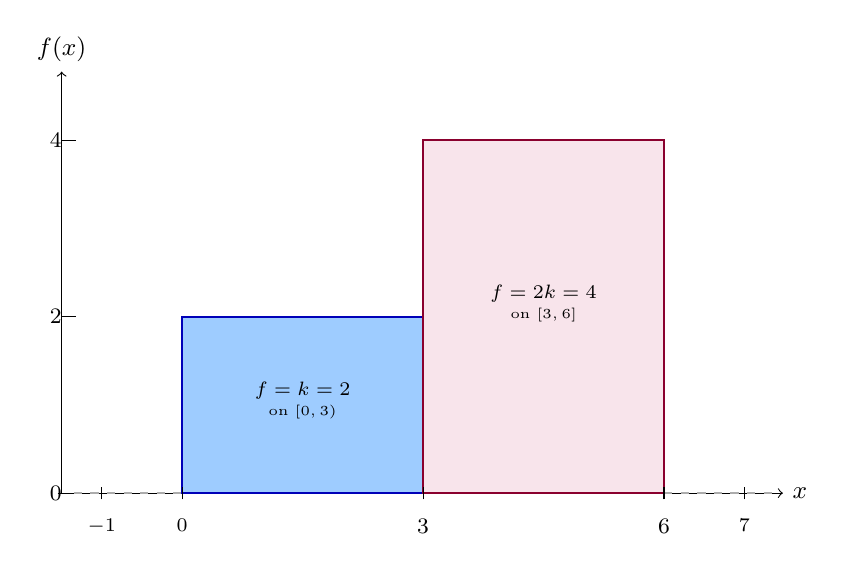
\begin{tikzpicture}[x=1.02cm,y=1.12cm]

  % Axes: $x\in[-1,7]$, $f$ up to $4$ (illustrative $k=2$)
  \draw[->] (-1.55, 0) -- (7.48, 0) node[right, font=\small] {$x$};
  \draw[->] (-1.5, 0) -- (-1.5, 4.78) node[above, font=\small] {$f(x)$};

  \foreach \yv in {0, 2, 4}{
    \draw (-1.5, \yv) -- (-1.32, \yv);
  }
  \foreach \yv/\Lb in {0/{$0$}, 2/{$2$}, 4/{$4$}}{
    \node[left=5pt, font=\footnotesize, inner sep=0pt] at (-1.32, \yv) {\Lb};
  }

  % Zero PDF on $(-\infty,0]$ and $(6,\infty)$ restricted to $[-1,0]$ and $[6,7]$
  \draw[thick, dashed, gray!65] (-1.35, 0) -- (0, 0);
  \draw[thick, dashed, gray!65] (6, 0) -- (7.4, 0);

  \fill[blue!52!cyan, opacity=0.38] (0, 0) rectangle (3, 2);
  \draw[thick, blue!72!black] (0, 0) rectangle (3, 2);

  \fill[purple!12, opacity=0.88] (3, 0) rectangle (6, 4);
  \draw[thick, purple!72!black] (3, 0) rectangle (6, 4);

  \foreach \xv in {-1, 0, 3, 6, 7}{
    \draw (\xv, -0.07) -- (\xv, 0.07);
  }

  \node[below=6pt, font=\scriptsize] at (-1, 0) {$-1$};
  \node[below=6pt, font=\scriptsize] at (0, 0) {$0$};
  \node[below=6pt, font=\footnotesize] at (3, 0) {$3$};
  \node[below=6pt, font=\footnotesize] at (6, 0) {$6$};
  \node[below=6pt, font=\scriptsize] at (7, 0) {$7$};

  \node[align=center, font=\scriptsize, inner sep=2pt] at (1.5, 1.05)
    {$f=k=2$\\[-1pt]{\tiny on $[0,3)$}};
  \node[align=center, font=\scriptsize, inner sep=2pt] at (4.5, 2.15)
    {$f=2k=4$\\[-1pt]{\tiny on $[3,6]$}};

\end{tikzpicture}\\[0.6em]

\noindent\footnotesize\textit{Illustration with $k=2$: steps at heights $k$ and $2k$; $f(x)=0$ on $[-1,0]$ and $[6,7]$. A valid pdf on $[0,6]$ needs $9k=1$, i.e.\ $k=\tfrac19$.}
\end{center}

\end{problem}

\begin{hint}
\begin{itemize}[leftmargin=*]
  \item Integrate over $[0,3]$ and $[3,6]$ and equate total area to $1$.
  \item Use $\int x f(x)\,dx$ split over the same pieces.
  \item $\mathrm{Var}(X)=E(X^2)-[E(X)]^2$.
\end{itemize}
\end{hint}

\begin{solution}
\textbf{(i)} A valid pdf must have total area $1$. Here the area is the sum of two rectangles:
\[
\int_0^3 k\,dx+\int_3^6 2k\,dx=3k+6k=9k.
\]
Thus $9k=1$, so $k=\frac19$.

\textbf{(ii)}
\[
E(X)=\int_0^{3}x\left(\frac{1}{9}\right)\,dx+\int_3^{6}x\left(\frac{2}{9}\right)\,dx.
\]
Evaluating,
\[
E(X)=\left[\frac{x^2}{18}\right]_0^3+\left[\frac{x^2}{9}\right]_3^6
=\frac{9}{18}+\left(\frac{36}{9}-\frac{9}{9}\right)=3{.}5.
\]
The mean is pulled to the right of the midpoint $3$ because the density is twice as high on $[3,6]$.

\textbf{(iii)} First compute
\[
E(X^{2})=\int_0^{3}x^{2}\left(\frac{1}{9}\right)\,dx+\int_3^{6}x^{2}\left(\frac{2}{9}\right)\,dx.
\]
This gives
\[
E(X^2)=\left[\frac{x^3}{27}\right]_0^3+\left[\frac{2x^3}{27}\right]_3^6=1+14=15.
\]
Therefore
\[
\mathrm{Var}(X)=E(X^2)-[E(X)]^2=15-(3{.}5)^2=\boxed{2{.}75}.
\]
\end{solution}

\begin{takeaways}
\item Rectangular strips make $k$ solvable by areas of rectangles.
\item Split integrals wherever the formula for $f$ changes.
\item Always use $E(X^{2})-[E(X)]^{2}$ for variance after $E(X^{2})$ is found.
\end{takeaways}
